\documentclass{report}
% PACKAGES %
\usepackage[english]{} % Sets the language
\usepackage[margin=2cm]{geometry} % Sets the margin size
\usepackage{graphicx} % Enhanced package for including graphics/figures
\usepackage{float} % Allows figures and tables to be floats
\usepackage{amsmath} % Enhanced math package prepared by the American Mathematical Society
\usepackage{amssymb} % AMS symbols package
\usepackage{bm} % Allows you to use \bm{} to make any symbol bold
\usepackage{verbatim} % Allows you to include code snippets
\usepackage{setspace} % Allows you to change the spacing between lines at different points in the document
\usepackage{parskip} % Allows you alter the spacing between paragraphs
\usepackage{multicol} % Allows text division into multiple columns
\usepackage{units} % Allows fractions to be expressed diagonally instead of vertically
\usepackage{booktabs,multirow,multirow} % Gives extra table functionality
\usepackage{enumerate}
\newcommand{\tab}{\-\hspace{1.5cm}}

% Set path to figure image files
\graphicspath{ {fig/} }

\begin{document}

\begin{center}
\textbf{\large Nuclear Engineering 150 -- Discussion Section}\\ 
\textbf{Notes}
\end{center}


%%%%%%%%%%%%%%%%%%%%%%%%%%%%%%%%%% TOPIC %%%%%%%%%%%%%%%%%%%%%%%%%%%%%%%%%%
\section*{Rate Independence of Absorption in $1/v$-absorbers} 

The rate of absorption in a $1/v$-absorber with microscopic absorption cross section $\sigma_a$ is independent of the energy of the neutrons involved in the reaction. This should make some intuitive sense. Neutrons with greater energies are traveling faster and so will tend to collide faster. At the same time, they also have lower cross sections (higher $v$, lower $\sigma = 1/v$) and so will be less likely to be absorbed. 

We can prove this independence more rigorously. We start by recalling the formula for a reaction rate, given energy dependent fluxes and cross sections. The reaction rate is the product of the macroscopic cross section of the material and the neutron flux. Since both cross section and flux can vary with energy, we must integrate over all possible energies to get a total reaction rate.

\begin{equation}
\label{reactionrate}
R = \int_0^{\infty} \Sigma_a(E) \, \phi(E) \, dE
\end{equation}

From this formula, we recall the definitions for both macroscopic cross section and flux. They are
$$ \Sigma_a(E) = N \sigma_a(E) \qquad\text{and}\qquad \phi(E) = n(E) v(E) $$
where $N$ is the number density of the absorbing material, $\sigma_a(E)$ is the microscopic absorption cross section of the material at energy $E$, $n(E)$ is the neutron number density at energy $E$, and $v(E)$ is the neutron speed given corresponding energy $E$. 

For $1/v$-absorbers, we note that the absorption cross section can be described given as
\begin{equation}
\label{microXS}
\sigma_a(E) = \frac{C}{\sqrt{E}}
\end{equation}
where $C$ is some constant of proportionality. Remembering that $E = \frac{1}{2}mv^2$, we can include the $\sqrt{\frac{m}{2}}$ factor in the constant $C$, and it becomes clear that indeed, $\sigma_a(E) \propto 1/v$. Now, we know that the $1/v$ behavior is dominant for low velocities and energies. In this case, let's write our constant $C$ in terms of one specific energy and the corresponding microscopic cross section. The choice of energy $E_0$ is arbitrary and so we will leave our formula in terms of the variable $E_0$ (frequently $E_0$ is chosen to be the thermal energy, $E_0 = 0.0253\text{ eV}$). In this case, we find
$$ \sigma_a(E_0) = \frac{C}{\sqrt{E_0}} $$
or
$$ C = \sigma_a(E_0)\sqrt{E_0} $$
Using this to replace $C$ in equation (\ref{microXS}), 
$$ \sigma_a(E) = \sigma_a(E_0)\sqrt{\frac{E_0}{E}} $$
Now that we have eliminated $C$, we can write this equation in terms of neutron speeds. If $E = \frac{1}{2}mv^2$ (and accordingly, $E_0 = \frac{1}{2}mv_0^2$), then
\begin{align*}
\sigma_a(E)	&= \sigma_a(E_0)\sqrt{\frac{\frac{1}{2}mv_0^2}{\frac{1}{2}mv^2}} \\
			&= \sigma_a(E_0)\sqrt{\frac{v_0^2}{v^2}} \\
			&= \sigma_a(E_0)\frac{v_0}{v}
\end{align*}
Explicitly noting the energy dependence of this velocity, the macroscopic cross section is
$$ \Sigma_a(E) = N \sigma_a(E_0)\frac{v_0}{v(E)} $$
We now return to our original equation for the reaction rate, equation (\ref{reactionrate}) and substitute in our explicit formulas for macroscopic cross section and flux.

$$ R = \int_0^{\infty} N \sigma_a(E_0)\frac{v_0}{v(E)} \, n(E) v(E) \, dE $$

In this equation, $N$, $\sigma_a(E_0)$, and $v_0$ are constants and can be brought outside of the integral, and the two instances of $v(E)$ cancel.

$$ R = N \sigma_a(E_0) v_0 \int_0^{\infty} n(E) \, dE $$

The integral of all number densities for all energies is just the total number of neutrons in the system, $n_0$. 
$$ n_0 = \int_0^{\infty} n(E) \, dE .$$
This formula can be put back in terms of macroscopic cross section and flux, both now constants ($\Sigma_a(E_0) = N \sigma_a(E_0)$ and $\phi_0 = v_0 n_0$).
\begin{align*}
R	&= N \sigma_a(E_0) v_0 n_0 \\
	&= \Sigma_a(E_0) \phi_0 \\
\end{align*}
This formula is clearly independent of energy, and suggests that the reaction rate will be constant regardless of the chosen energy. Perhaps more surprisingly, for $1/v$-absorbers the reaction rate is the same whether the neutrons are all at one energy or covering a range of energies. Any increase in the neutron flux is compensated for exactly by a decrease in cross section, and vice-versa.


\newpage
%%%%%%%%%%%%%%%%%%%%%%%%%%%%%%%%%% TOPIC %%%%%%%%%%%%%%%%%%%%%%%%%%%%%%%%%%
\section*{The Maxwell-Boltzmann Distribution for Neutrons} 

The fundamental assumption behind the Maxwell-Boltzmann (MB) distribution is that particles behave like an ideal gas; specifically
\begin{itemize}
\item interactions are classical (collisions are instantaneous and elastic)
\item the surrounding environment is thermal
\end{itemize}
While this might seem like a stretch given the various other processes we have discussed (fission, radiative capture, and inelastic scattering) the distribution still does a reasonable job approximating the thermal neutron energy distribution in reactors. Remember that reactors have significant quantities of moderator and so neutron-moderator collisions are generally elastic; if our reactor was pure uranium, this model would be far less effective.

Still, we are making some big assumptions, so let's be very explicit. Modeling the thermal distribution of neutrons with the MB distribution assumes
\begin{enumerate}
\item no absorption
\item no leakage
\item no sources
\end{enumerate}
\-\\
Now, we can look at the distribution itself. We won't derive it here, but using statistical physics it can be shown that
$$ M(v) = 4 \pi v^2 \left(\frac{m}{2 \pi k_B T} \right)^{3/2} e^{\frac{-m v^2}{2 k_B T}} ,$$
or equivalently (as a distribution for energies)
$$ M(E) = 2\sqrt{\frac{E}{\pi}}\left(\frac{1}{kT}\right)^{3/2} e^{-\frac{E}{kT}} .$$
\begin{figure}[h]
\begin{multicols}{2}\begin{enumerate}[(a)]
\item 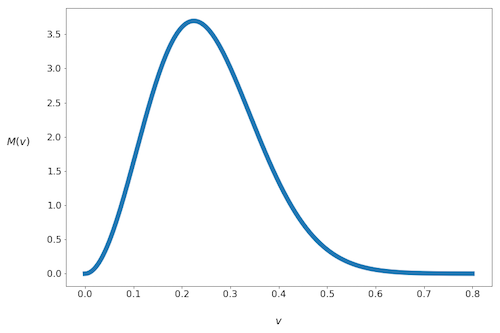
\includegraphics[width=8cm]{mb-dist_v.png}
\item 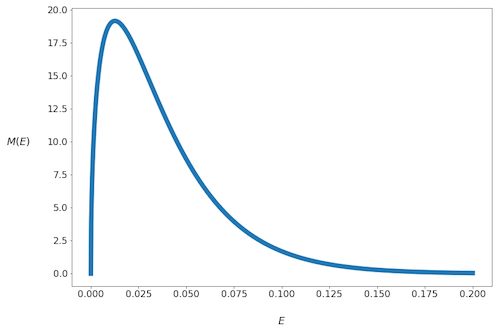
\includegraphics[width=8cm]{mb-dist_E.png}
\end{enumerate}\end{multicols}
\caption{(a) The MB distribution as a function of velocity, compared to (b) the distribution as a function of energy.}
\end{figure}





\end{document}

